\subsection{Molten Salt Reactors}

\begin{frame}
\frametitle{Potential Generation IV reactor systems \cite{abram_generation-iv_2008}}
\begin{figure}[t]
	\vspace*{-0.1in}
	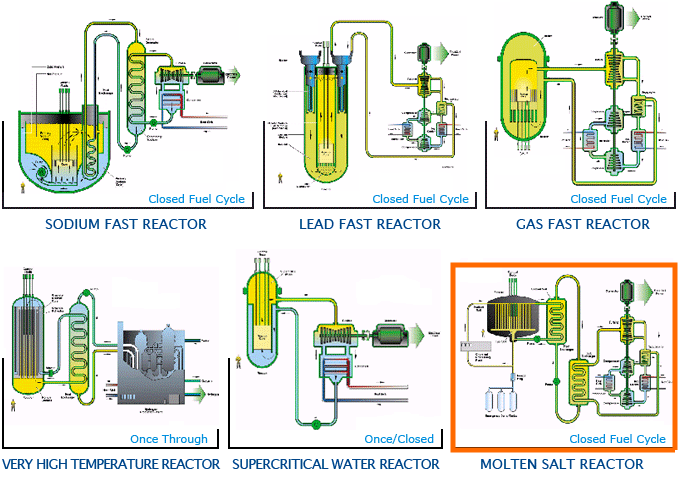
\includegraphics[height=0.7\textwidth]{./images/6_types.png}
	\caption{\gls{MSR} design}
\end{figure}            
\end{frame}


\begin{frame}
\frametitle{MSR (Molten Salt Reactor) types}
\begin{overlayarea}{\linewidth}{20\baselineskip}
\begin{block}{Stationary Fuel}<1-4>
	\begin{enumerate}
		\item Graphite block with TRISO fuel, clean salt works as 
		coolant (Fluoride-Salt-Cooled High-Temperature 
		Reactor (FHR))
		\item Plate Fuel: hexagonal fuel assembly is similar in shape to a typical sodium-cooled reactor
		\item Fuel Inside Radial Moderator (FIRM)
		\item Liquid fuel salt inside fuel rods cooled by clean salt 
		(Moltex Stable Salt Reactor)
	\end{enumerate}
\end{block}

\begin{block}{Mobile Fuel}<2-4>
	\begin{enumerate}
		\item<2-4> Mobile solid fuel elements (pebbles) cooled by 
		clean salt (PB-FHR)
		\item<3-4> Non-circulating liquid fuel salt (TerraPower \gls{MCFR}) 
		\item<4> \textbf{Circulating liquid fuel salt} which also works 
		as coolant (\gls{MSBR})
	\end{enumerate}
\end{block}
\end{overlayarea}
\end{frame}


%\begin{frame}
%\frametitle{Stationary and Mobile Solid fuel}
%\vspace*{-0.1in}
%\begin{figure}[t]
%	\hspace*{-0.35in}
%	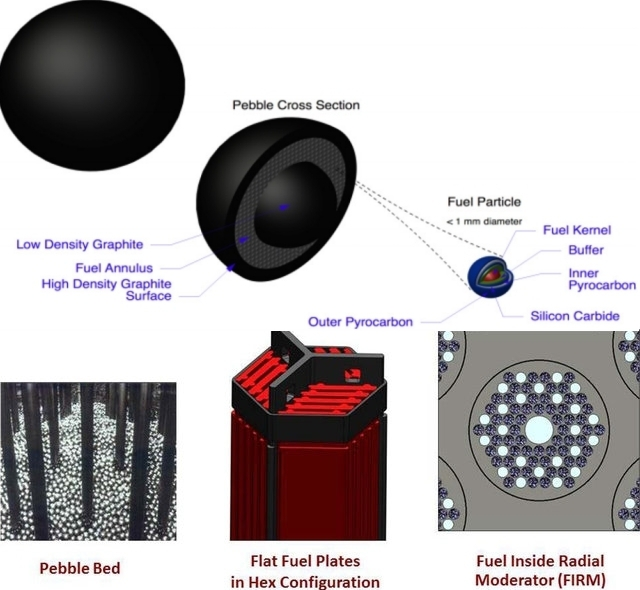
\includegraphics[height=0.63\textwidth]{./images/solid_fuel.jpg}
%	\caption{TRISO fuel particle (top) and FHR fuel designs (bottom) 
%	\cite{forsberg_basis_2016}.} 
%\end{figure}   
%\end{frame}

\begin{frame}
\frametitle{Mobile, Non-Circulating, Liquid Fuel}
\begin{figure}[t]
\vspace*{-0.1in}
\hspace*{-0.35in}
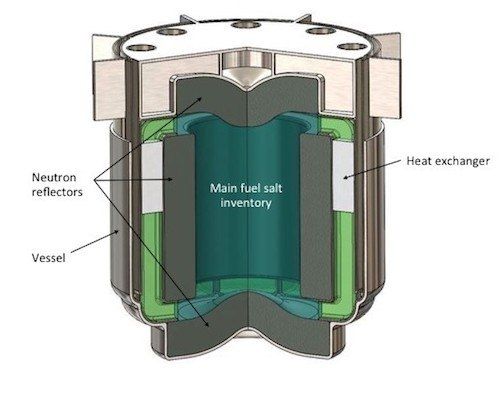
\includegraphics[height=0.6\textwidth]{./images/mcfr-crossection.jpg}
\caption{The TerraPower MCFR is an example of reactor design with 
\textbf{liquid, mobile, non-circulating} chloride salt fuel 
\cite{doene_southern_2018}.}
\end{figure}   

\end{frame}


\begin{frame} % Add another slide with red rectangular around reprocessing system
\frametitle{Mobile, Circulating, Liquid Fuel}
\vspace{-2mm}
\begin{figure}[t]
      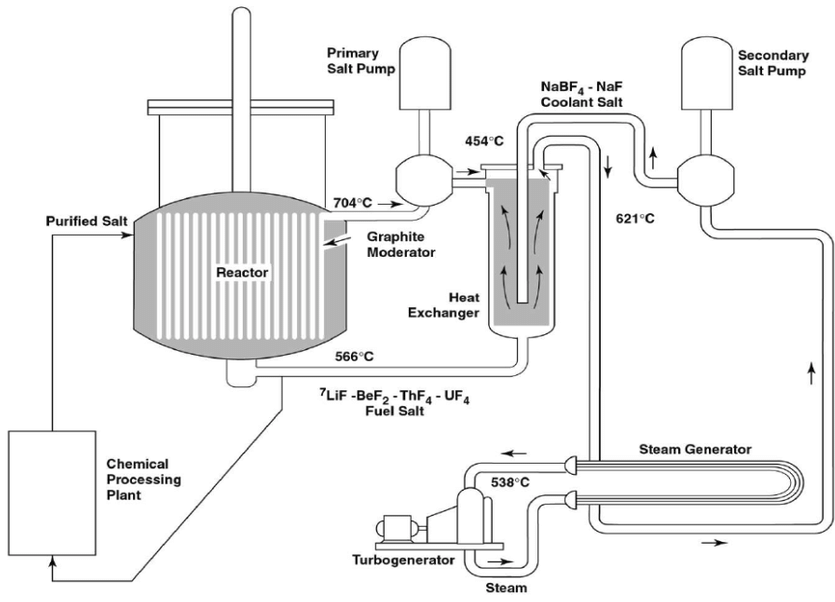
\includegraphics[height=0.6\textwidth]{./images/msbr_scheme.png}
	\caption{The \gls{MSBR} is an example of reactor design with 
	\textbf{liquid, mobile, circulating} fluoride salt fuel 
	(reproduced from Rosenthal \emph{et al.} 
	\cite{rosenthal_molten-salt_1970}).}
\end{figure}   

\end{frame}


\subsection{Motivation}

\begin{frame}
\frametitle{Why Molten Salt Reactors with circulating fuel?}
\begin{block}{Liquid-fueled \gls{MSR} designs have following \textbf{potential} advantages:}
	\begin{enumerate}
		\itemsep1em
		\item High coolant temperature (600-750$^{\circ}$C) 
		$\Rightarrow$ potentially high thermal efficiency, process 
		heat for chemical industry
		\item Fuel diversity ($^{235}$U, $^{233}$U, Thorium, U/Pu)
		\item Strong negative fuel temperature feedback 
		\item Passive safety $\Rightarrow$ fuel drains into tanks 
		in emergency
		\item High fuel utilization $\Rightarrow$ reduced spent fuel 
		generation
		\item<2> \textbf{On-line (continuous) fuel reprocessing potentially  
		allows to avoid Xenon-135 poisoning} $\Rightarrow$ exceptional 
		performance during load following
	\end{enumerate}
\end{block}

\end{frame}

\begin{frame}
\frametitle{What is Xenon-135 poisoning?}
\animategraphics[loop,controls,width=1.07\linewidth]{0.5}{./images/anime/xe_pois-}{0}{11}
\end{frame}

\begin{frame}
\frametitle{Why load following nuclear reactor is a game changer?}
sdfdf
\end{frame}



\subsection{Research objectives}

\begin{frame}
  \frametitle{Research objectives of purposed work}
                  \vspace*{-0.05in}
      The main objective of the proposed work is to develop the on-line  reprocessing simulation package, SaltProc, for liquid-fueled MSR depletion simulations.
     \begin{block}{SaltProc desired capabilities:}<1-6>
         \begin{enumerate}
         		%\itemsep1em
                \item \textbf{Realistic} multi-component fuel 
                reprocessing 
                system modeling
                \item \textbf{Variable} extraction efficiency support
                \item<2-6> Reactivity control by \textbf{changing geometry} of 
                the core during simulation
                \item<3-6> \textbf{Open-source} with continuous tests and 
                automatic documentation system 
         \end{enumerate}
      \end{block}
            \vspace{-0.1in}
	\begin{block}{SaltProc demonstration and validation}<4-6>
		\begin{enumerate}
			\item<4-6> \textbf{Lifetime-long (60 years)} depletion with ideal/realistic $\epsilon_e$
			\item<5-6> Short-term (3-7 days) depletion for the \gls{TAP} concept \textbf{during load-following}
			\item<6> Safety parameters (thermal feedback coefficient, control rod worth, power 
			axial offset) \textbf{evolution during operation}
		\end{enumerate}
	\end{block}
\end{frame}
